\chapter{Rendimiento observado de los alumnos}\label{chapter:rendimiento}
\addcontentsline{toc}{chapter}{Rendimiento observado de los alumnos}

\section{Calificaciones obtenidas (Grade)}

La primera medida de rendimiento que tendremos en cuenta son las calificaciones de los grupos de prácticas. Nótese que estas calificaciones no son la evaluación final de cada grupo, sino la nota de la práctica cuya evolución se está analizando. Esta es la parte más subjetiva de la evaluación del rendimiento de cada alumno pues implica la participación del profesor y la toma en consideración de otros factores, además de los registrados en el servidor como puede ser la calidad de la memoria de la práctica. Las calificaciones muestran una distribución normal a lo largo de estos siete años de registros, ligeramente inclinada a la derecha porque las notas medias de esta asignatura suelen ser altas tal y como puede verse en la Figura \ref{fig:densityplotachiever}.

\begin{figure}[H]
    \centering
    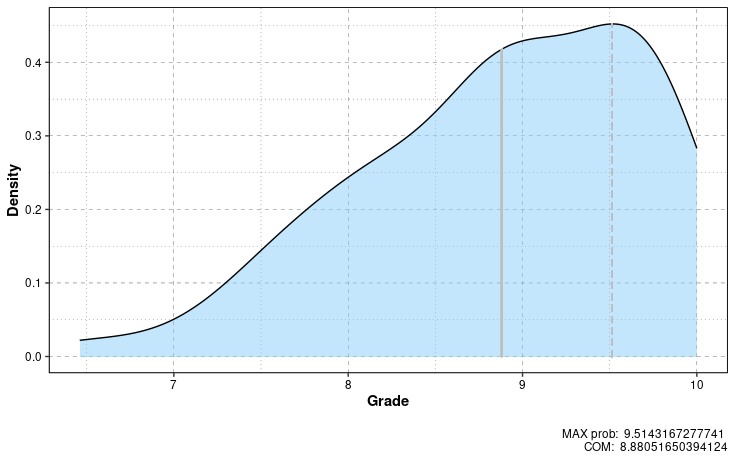
\includegraphics[width=0.70\textwidth]{rendimiento/densitygrade.png}
    \caption{Función de densidad de probabilidad de las calificaciones obtenidas por los distintos grupos de prácticas.}
    \label{fig:densityplotachiever}
\end{figure}

Además, la media está bastante balanceada (Figuras \ref{fig:boxplotresidualsachiever} y \ref{fig:histogramresidualsachiever}) y no se detecta la presencia de outliers (Figura \ref{fig:outliersgrade}).

\begin{figure}[H]
\centering
\subfloat[Boxplot de los residuos de las calificaciones.]{\label{fig:boxplotresidualsachiever}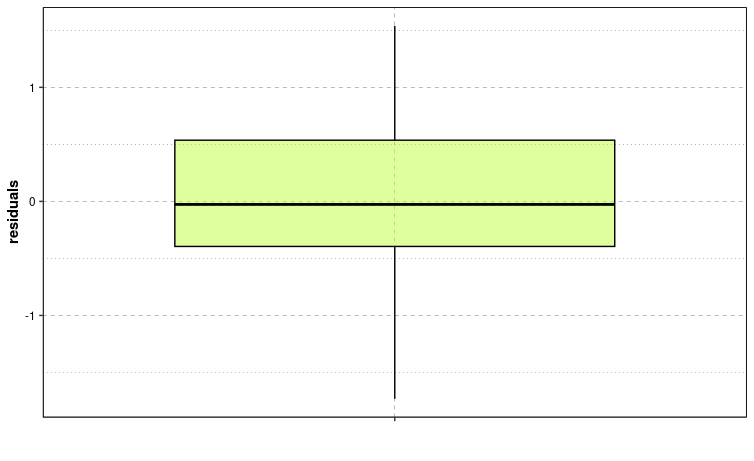
\includegraphics[width=0.47\textwidth]{rendimiento/residualsgrade.png}}\qquad
\subfloat[Histograma de los residuos de las calificaciones.]{\label{fig:histogramresidualsachiever}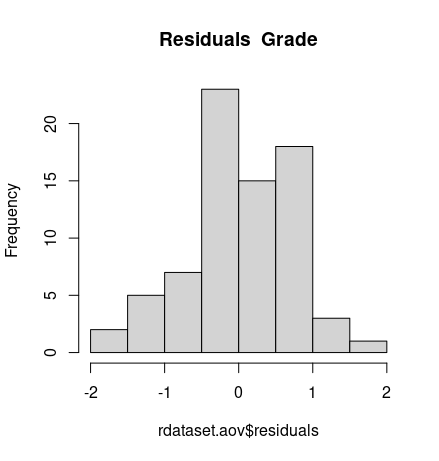
\includegraphics[width=0.47\textwidth]{rendimiento/histogramgrade.png}}
\caption{Distribución de los residuos de las calificaciones.}
\label{fig:achiever}
\end{figure}

\begin{figure}[H]
    \centering
    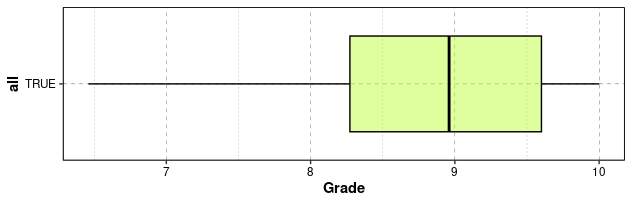
\includegraphics[width=0.60\textwidth]{rendimiento/outliersgrade.png}
    \caption{Distribución de las calificaciones obtenidas por los distintos grupos de alumnos inicial.}
    \label{fig:outliersgrade}
\end{figure}

Más aún, la regresión es muy aceptable (Figura \ref{fig:q-qsessionsachiever}).

\begin{figure}[H]
    \centering
    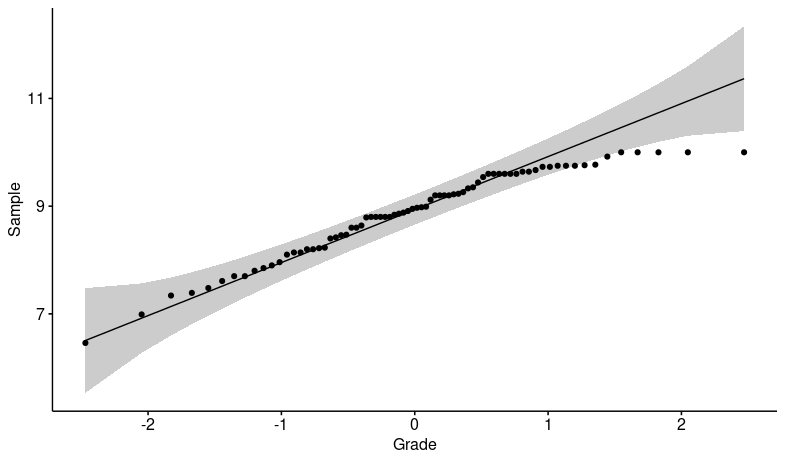
\includegraphics[width=0.75\textwidth]{rendimiento/qqplotgrade.png}
    \caption{Gráfico Q-Q de las calificaciones.}
    \label{fig:q-qsessionsachiever}
\end{figure}

A continuación se realizará un estudio por años de las calificaciones obtenidas. El boxplot de las calificaciones por años puede verse en la Figura \ref{fig:boxplotachieveryear}. Como se puede observar, los datos recogidos muestran una variación muy perceptible en las notas a lo largo de los años. De hecho, los tests estadísticos ratifican que hay diferentes significativas entre ellas. Tras realizar el test ANOVA de un factor (resultados en el Cuadro \ref{tab:ANOVAachiever}) obtenemos $p = 0.00143 < 0.05$. Además, tras realizar el test de Kruskal-Wallis se obtiene $p-value = 0.01534$. Un análisis posterior por pares de Tukey muestra las diferencias entre los años (resultados en el Cuadro \ref{tab:Tukeyachiever}). Podemos ver que el año 2017 es el principal elemento de disrupción, pero por poco margen. Lo mismo indica el análisis de los intervalos de confianza de la Figura \ref{fig:confidenceachiever}.

\begin{figure}[H]
    \centering
    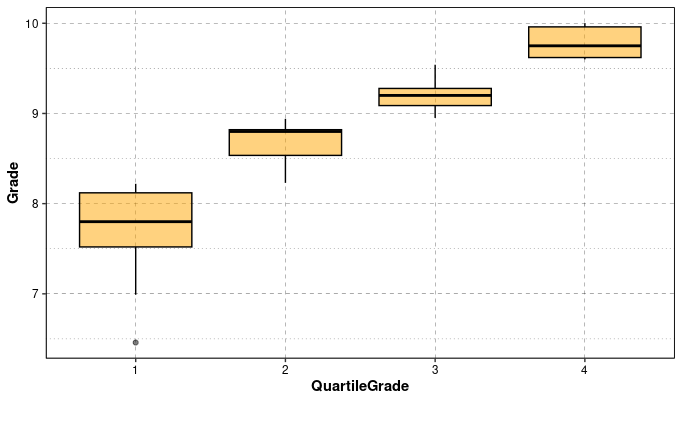
\includegraphics[width=0.8\textwidth]{rendimiento/boxplotgrade.png}
    \caption{Boxplot de las calificaciones por año.}
    \label{fig:boxplotachieveryear}
\end{figure}

% latex table generated in R 4.3.0 by xtable 1.8-4 package
% Sun Jun  4 18:14:08 2023
\begin{table}[H]
\centering
\caption{Resultados del test ANOVA de un solo factor (calificaciones).}
\label{tab:ANOVAachiever}
% latex table generated in R 4.3.0 by xtable 1.8-4 package
% Mon Jun  5 21:06:19 2023
\centering
\begin{tabular}{lrrrrr}
  \hline
 & Df & Sum Sq & Mean Sq & F value & Pr($>$F) \\ 
  \hline
Grade & 6 & 13.05 & 2.18 & 4.11 & 0.0014 \\ 
  Residuals            & 67 & 35.47 & 0.53 &  &  \\ 
   \hline
\end{tabular}
\end{table}

% latex table generated in R 4.3.0 by xtable 1.8-4 package
% Sun Jun  4 18:14:38 2023
\begin{table}[H]
\centering
\caption{Test HSD de Tukey (Honestly-significance-difference) de las calificaciones por años.}
\label{tab:Tukeyachiever}
\begin{tabular}{rrrrr}
  \hline
 & diff & lwr & upr & p adj \\ 
  \hline
Y2016-Y2015 & 0.18 & -0.87 & 1.22 & 1.00 \\ 
  Y2017-Y2015 & -1.35 & -2.52 & -0.19 & 0.01 \\ 
  Y2018-Y2015 & -0.45 & -1.47 & 0.57 & 0.83 \\ 
  Y2019-Y2015 & -0.24 & -1.23 & 0.76 & 0.99 \\ 
  Y2020-Y2015 & -0.10 & -1.06 & 0.85 & 1.00 \\ 
  Y2021-Y2015 & 0.22 & -0.70 & 1.14 & 0.99 \\ 
  Y2017-Y2016 & -1.53 & -2.70 & -0.36 & 0.00 \\ 
  Y2018-Y2016 & -0.63 & -1.64 & 0.39 & 0.51 \\ 
  Y2019-Y2016 & -0.41 & -1.41 & 0.58 & 0.87 \\ 
  Y2020-Y2016 & -0.28 & -1.24 & 0.68 & 0.97 \\ 
  Y2021-Y2016 & 0.05 & -0.88 & 0.97 & 1.00 \\ 
  Y2018-Y2017 & 0.90 & -0.24 & 2.05 & 0.21 \\ 
  Y2019-Y2017 & 1.12 & -0.00 & 2.24 & 0.05 \\ 
  Y2020-Y2017 & 1.25 & 0.16 & 2.34 & 0.01 \\ 
  Y2021-Y2017 & 1.57 & 0.52 & 2.63 & 0.00 \\ 
  Y2019-Y2018 & 0.21 & -0.75 & 1.18 & 0.99 \\ 
  Y2020-Y2018 & 0.34 & -0.59 & 1.28 & 0.92 \\ 
  Y2021-Y2018 & 0.67 & -0.22 & 1.56 & 0.27 \\ 
  Y2020-Y2019 & 0.13 & -0.78 & 1.04 & 1.00 \\ 
  Y2021-Y2019 & 0.46 & -0.41 & 1.32 & 0.68 \\ 
  Y2021-Y2020 & 0.33 & -0.50 & 1.15 & 0.89 \\ 
   \hline
\end{tabular}
\end{table}

\begin{figure}[H]
    \centering
    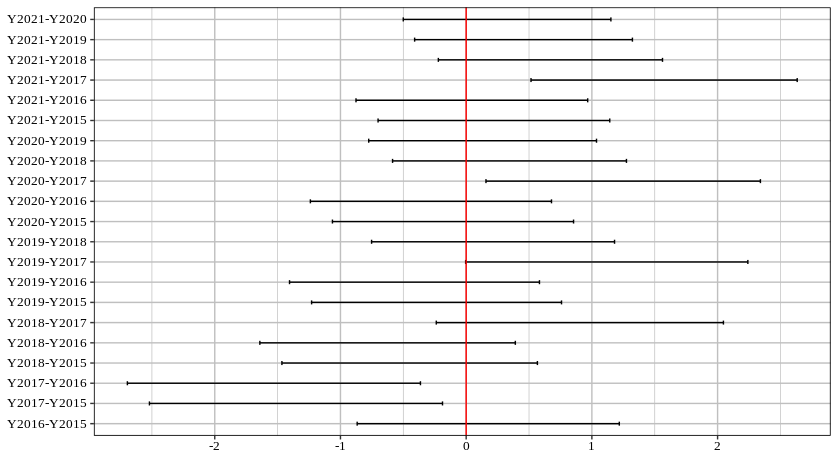
\includegraphics[width=0.80\textwidth]{rendimiento/confidencegrade.png}
    \caption{Intervalos de confianza de las calificaciones por años.}
    \label{fig:confidenceachiever}
\end{figure}

\section{Número total de problemas resueltos (p)}

Podemos observar que ha habido variaciones perceptibles durante los distintos cursos académicos estudiados, siendo un caso especial el año $2018$ en el que hubo muchos grupos que no resolvieron todos los problemas (Figura \ref{fig:boxplotperformer}).

\begin{figure}[H]
    \centering
    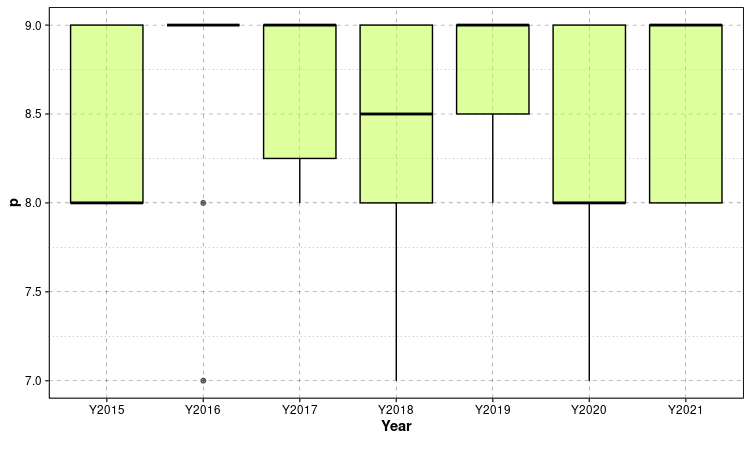
\includegraphics[width=0.8\textwidth]{rendimiento/boxplotp.png}
    \caption{Boxplot del número de problemas resueltos por año.}
    \label{fig:boxplotperformer}
\end{figure}

Sin embargo, las diferencias entre las medias no son estadísticamente significativas (considerando un nivel de significancia de $0.05$) tal y como puede verse en el Cuadro \ref{tab:ANOVAperformer} ($p = 0.2835 > 0.05$). Además, si consideramos el test estadístico de Kruskal-Wallis llegamos a la misma conclusión ($p-value = 0.365 > 0.05$). Así pues, se concluye que el número de problemas resueltos por años es uniforme (cualquier variación es debida al azar).

Además, realizando un test de Tukey por pares de años (Cuadro \ref{tab:Tukeyperformer}) se observa que todos los pares pueden considerarse estadísticamente iguales. La Figura \ref{fig:confidenceperformer} muestra los intervalos de confianza de todas las diferencias entre las distintas parejas de años.

% latex table generated in R 4.3.0 by xtable 1.8-4 package
% Tue Jun  6 20:27:28 2023
\begin{table}[H]
\centering
\caption{Resultados del test ANOVA de un solo factor (número de problemas resueltos).}
\label{tab:ANOVAperformer}
\begin{tabular}{lrrrrr}
  \hline
 & Df & Sum Sq & Mean Sq & F value & Pr($>$F) \\ 
  \hline
p & 6 & 2.91 & 0.48 & 1.27 & 0.2835 \\ 
  Residuals            & 67 & 25.58 & 0.38 &  &  \\ 
   \hline
\end{tabular}
\end{table}

% latex table generated in R 4.3.0 by xtable 1.8-4 package
% Tue Jun  6 20:27:48 2023
\begin{table}[ht]
\centering
\caption{Test HSD de Tukey (Honestly-significance-difference) del número de problemas resueltos por año.}
\label{tab:Tukeyperformer}
\begin{tabular}{rrrrr}
  \hline
 & diff & lwr & upr & p adj \\ 
  \hline
Y2016-Y2015 & 0.22 & -0.66 & 1.11 & 0.99 \\ 
  Y2017-Y2015 & 0.22 & -0.77 & 1.21 & 0.99 \\ 
  Y2018-Y2015 & -0.04 & -0.91 & 0.82 & 1.00 \\ 
  Y2019-Y2015 & 0.28 & -0.56 & 1.13 & 0.95 \\ 
  Y2020-Y2015 & -0.29 & -1.11 & 0.52 & 0.93 \\ 
  Y2021-Y2015 & 0.18 & -0.60 & 0.96 & 0.99 \\ 
  Y2017-Y2016 & 0.00 & -0.99 & 0.99 & 1.00 \\ 
  Y2018-Y2016 & -0.27 & -1.13 & 0.60 & 0.96 \\ 
  Y2019-Y2016 & 0.06 & -0.78 & 0.90 & 1.00 \\ 
  Y2020-Y2016 & -0.51 & -1.33 & 0.30 & 0.48 \\ 
  Y2021-Y2016 & -0.04 & -0.82 & 0.74 & 1.00 \\ 
  Y2018-Y2017 & -0.27 & -1.24 & 0.70 & 0.98 \\ 
  Y2019-Y2017 & 0.06 & -0.89 & 1.01 & 1.00 \\ 
  Y2020-Y2017 & -0.51 & -1.44 & 0.41 & 0.63 \\ 
  Y2021-Y2017 & -0.04 & -0.94 & 0.86 & 1.00 \\ 
  Y2019-Y2018 & 0.33 & -0.49 & 1.15 & 0.89 \\ 
  Y2020-Y2018 & -0.25 & -1.04 & 0.54 & 0.96 \\ 
  Y2021-Y2018 & 0.22 & -0.53 & 0.98 & 0.97 \\ 
  Y2020-Y2019 & -0.57 & -1.34 & 0.20 & 0.28 \\ 
  Y2021-Y2019 & -0.10 & -0.84 & 0.63 & 1.00 \\ 
  Y2021-Y2020 & 0.47 & -0.23 & 1.17 & 0.40 \\ 
   \hline
\end{tabular}
\end{table}

\begin{figure}[H]
    \centering
    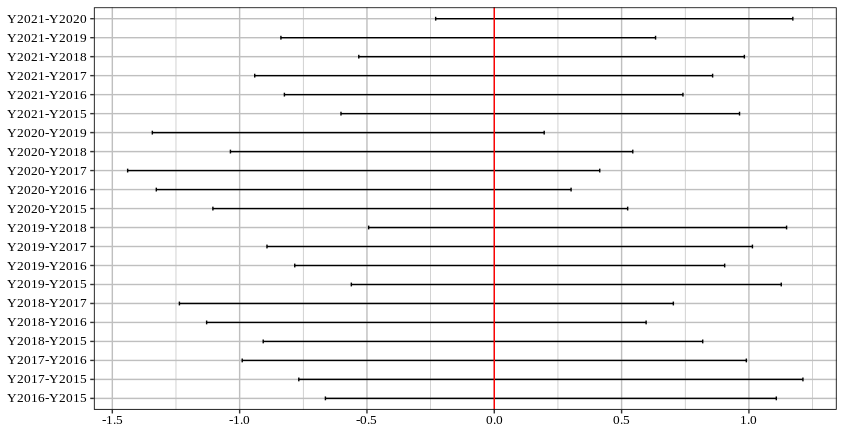
\includegraphics[width=0.80\textwidth]{rendimiento/confidencep.png}
    \caption{Intervalos de confianza del número de problemas resueltos por años.}
    \label{fig:confidenceperformer}
\end{figure}

Por último, podemos concluir que la variable número de problemas resueltos por año (\emph{p}) no es muy normal en tanto que varía muy poco y es discreta (Figuras \ref{fig:countp} y \ref{fig:densityp}).

\begin{figure}[H]
\centering
\subfloat[Número de grupos que han resuelto una determinada cantidad de problemas.]{\label{fig:countp}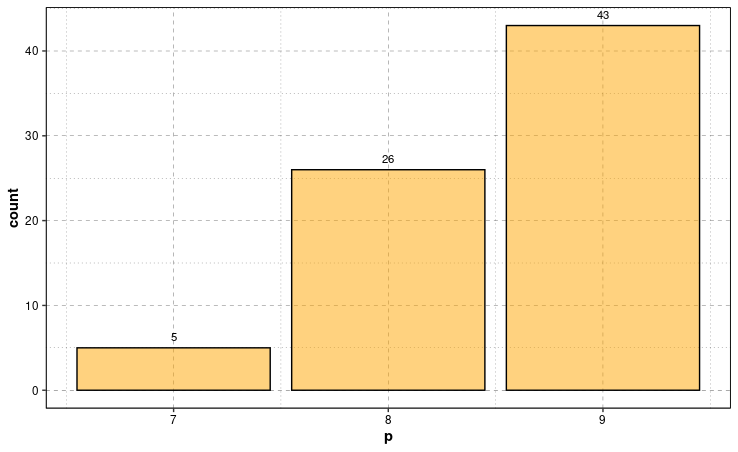
\includegraphics[width=0.47\textwidth]{rendimiento/countp.png}}\qquad
\subfloat[Función de densidad de probabilidad del número de problemas resueltos.]{\label{fig:densityp}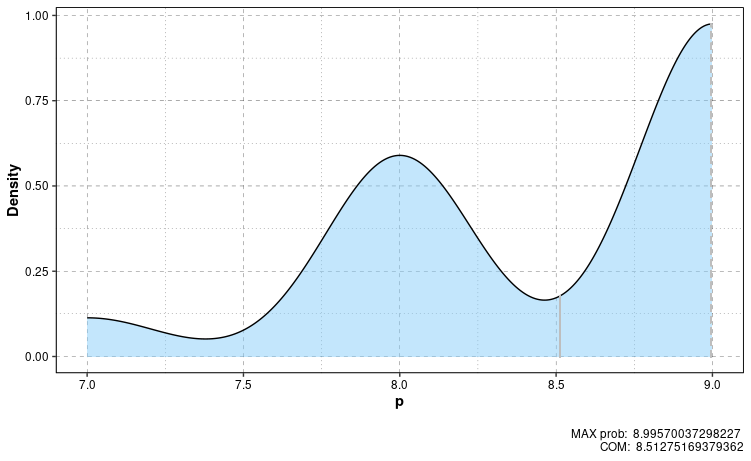
\includegraphics[width=0.47\textwidth]{rendimiento/densityp.png}}
\caption{Distribución del número de problemas resueltos por cada grupo de alumnos.}
\label{fig:normalityp}
\end{figure}

\section{Finalizar la práctica (ft)}

Como vemos en la Figura \ref{fig:densityplotft}, el punto de finalización de la práctica normalizado tiende a estar cerca del final de la misma.

 \begin{figure}[H]
    \centering
    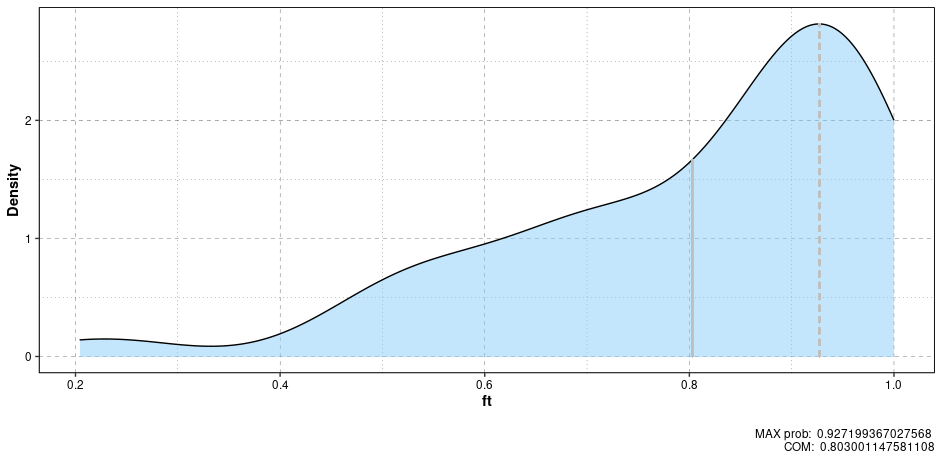
\includegraphics[width=0.70\textwidth]{rendimiento/densityft.png}
    \caption{Función de densidad de probabilidad del momento en el que los distintos grupos de prácticas finalizan la práctica.}
    \label{fig:densityplotft}
\end{figure}

\section{Número de sesiones realiazadas (s)}

El número de sesiones realizadas por los diferentes grupos de prácticas se ha analizado con anterioridad. En la Sección \ref{sec:NormalityNumSessions} vimos que seguía una distribución casi normal. Además, vimos que el número de sesiones sigue la misma distribución de probabilidad en cada uno de los cursos académicos considerados (Sección \ref{sec:ANOVANumSessions}).

%\section{Sesiones perdidas durante un problema}

%Con frecuencia ocurre que los alumnos, cuando intentan resolver un problema y no lo consiguen, saltan, curiosamente, a sesiones en otros problemas más complejos, los cuales, obviamente, tampoco pueden resolver.

%\textbf{Falta gráfica.}

%Este hábito es más frecuente de lo que parece y mantiene mucha variación en cada problema, sobre todo es más fuerte al comienzo de las prácticas, pero es homogéneo año tras año (ANOVA p=0.746, KW p=0.9) y se puede decir que está presente en la mayoría de los grupos. Aunque la mediana sea 0, casi todos los grupos (80\%) exhiben este comportamiento en algún momento.

%\textbf{Referenciar tabla ya existente}.

%\textbf{Falta gráfica.}

\section{Abrir un problema por primera vez (ot)}

Momento exacto en el que se consigue abrir cada problema por primera vez en el servidor, normalizado para poder compararlo (se normaliza porque la duración de la práctica no es la misma todos los años). Como podemos ver en su función de densidad (Figura \ref{fig:densityplotnewcomer}) y en su gráfico Q-Q (Figura \ref{fig:q-qot}), se aproxima a una distribución normal, un poco ladeada hacia la derecha. Esto puede deberse a que los distintos equipos tienden a abrir los problemas cuando se va aproximando la fecha de entrega de la práctica.

\begin{figure}[H]
    \centering
    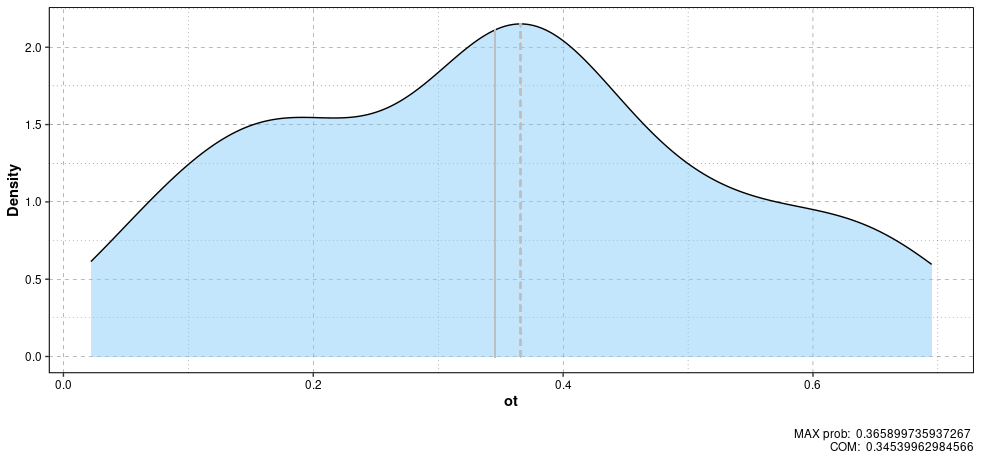
\includegraphics[width=0.70\textwidth]{rendimiento/densityot.png}
    \caption{Función de densidad de probabilidad del momento en el que los distintos grupos de prácticas abren por primera vez un problema.}
    \label{fig:densityplotnewcomer}
\end{figure}

\begin{figure}[H]
    \centering
    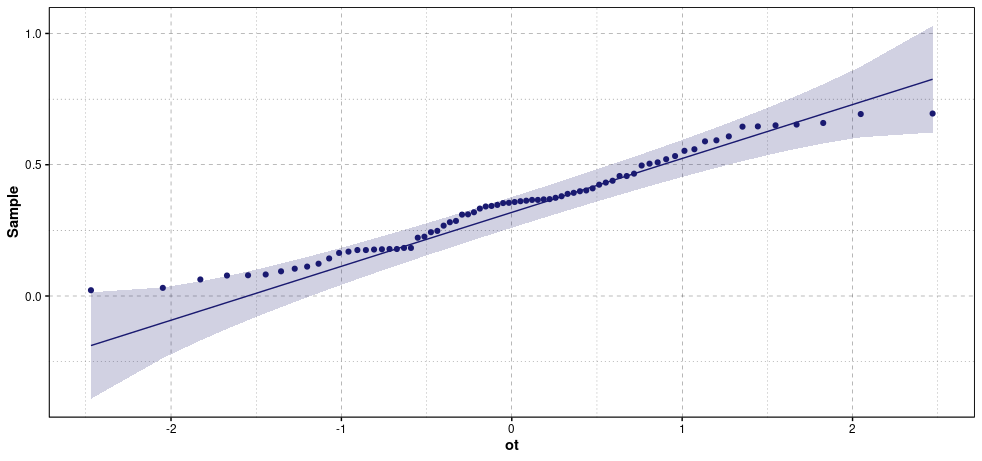
\includegraphics[width=0.75\textwidth]{rendimiento/qqplotot.png}
    \caption{Gráfico Q-Q del instante temporal en el que se abren los problemas por primera vez normalizado.}
    \label{fig:q-qot}
\end{figure}

En las Figuras \ref{fig:boxplotresidualsnewcomer} y \ref{fig:histogramresidualsnewcomer} pueden verse el boxplot de los residuos y el histograma de los mismos respectivamente.

\begin{figure}[H]
\centering
\subfloat[Boxplot de los residuos del instante temporal en el que se abren los problemas por primera vez.]{\label{fig:boxplotresidualsnewcomer}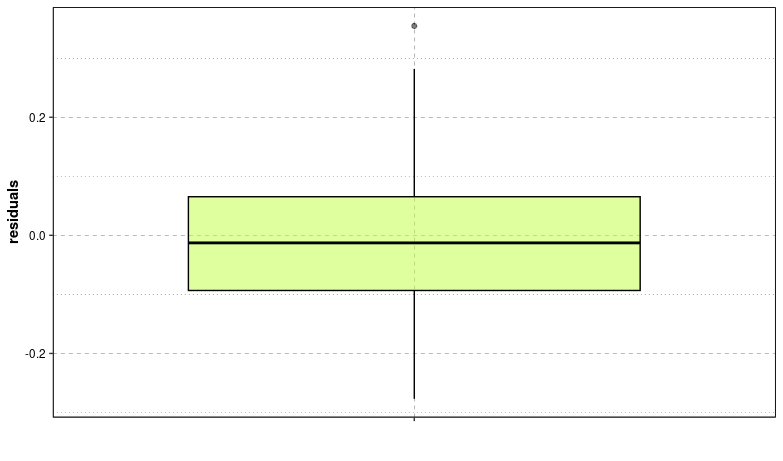
\includegraphics[width=0.47\textwidth]{rendimiento/residualsot.png}}\qquad
\subfloat[Histograma de los residuos del momento en el que se abren los problemas por primera vez.]{\label{fig:histogramresidualsnewcomer}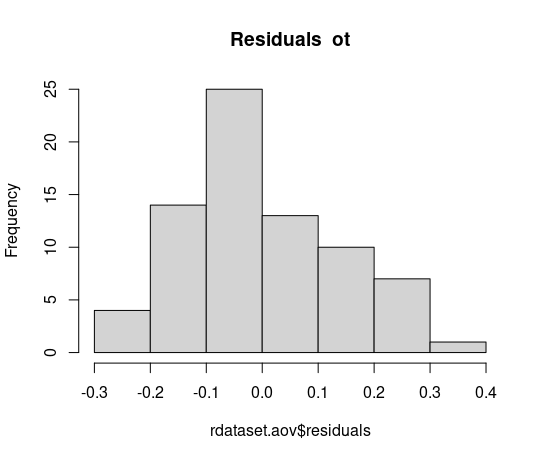
\includegraphics[width=0.47\textwidth]{rendimiento/histogramot.png}}
\caption{Distribución de los residuos del momento en el que se abren los problemas por primera vez.}
\label{fig:newcomer}
\end{figure}

Si realizamos una segmentación por años, podemos ver que la media de esta medida de rendimiento puede variar según el año que estemos considerando (Figura \ref{fig:boxplotnewcomer}). El test ANOVA de un sólo factor ha confirmado lo observado (se ha obtenido $p = 4.05e-06 < 0.05$ como puede verse en el Cuadro \ref{tab:ANOVAnewcomer}). Igualmente, el test de Kruskal-Wallis coincide con lo anteriormente visto ($p-value = 4.633e-05 < 0.05$).

\begin{figure}[H]
    \centering
    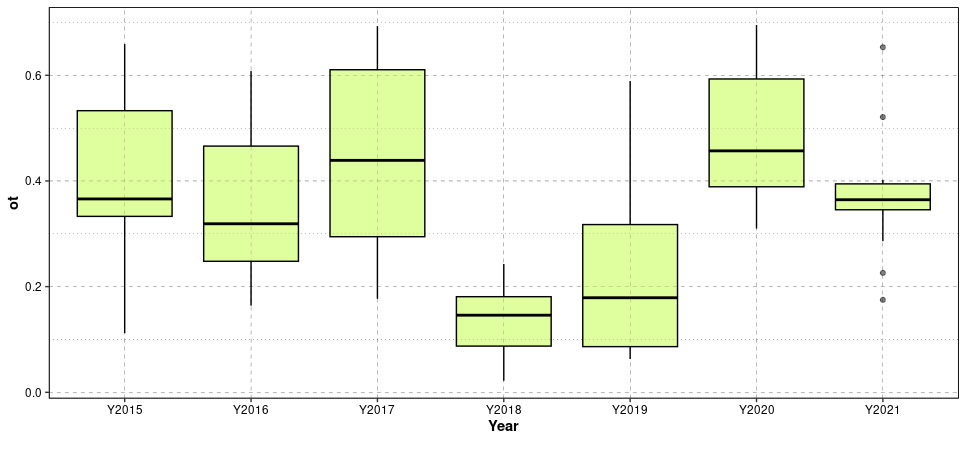
\includegraphics[width=0.8\textwidth]{rendimiento/boxplotot.png}
    \caption{Boxplot del momento en el que se abre un problema por primera vez por año.}
    \label{fig:boxplotnewcomer}
\end{figure}

% latex table generated in R 4.3.0 by xtable 1.8-4 package
% Sun Jun 11 18:57:16 2023
\begin{table}[H]
\centering
\caption{Resultados del test ANOVA de un solo factor (momento en el que se abre un problema por primera vez).}
\label{tab:ANOVAnewcomer}
\begin{tabular}{lrrrrr}
  \hline
 & Df & Sum Sq & Mean Sq & F value & Pr($>$F) \\ 
  \hline
ot & 6 & 0.93 & 0.15 & 7.43 & 4.05e-06 \\ 
  Residuals            & 67 & 1.40 & 0.02 &  &  \\ 
   \hline
\end{tabular}
\end{table}

Tras realizar el test de Tukey por pares se ha visto que claramente hay años con distribuciones diferentes de esta variable (Cuadro \ref{tab:Tukeynewcomer} y Figura \ref{fig:confidencenewcomer}).

% latex table generated in R 4.3.0 by xtable 1.8-4 package
% Sun Jun 11 18:57:48 2023
\begin{table}[H]
\centering
\caption{Test HSD de Tukey (Honestly-significance-difference) del momento exacto en el que se abre un problema por primera por año.}
\label{tab:Tukeynewcomer}
\begin{tabular}{rrrrr}
  \hline
 & diff & lwr & upr & p adj \\ 
  \hline
Y2016-Y2015 & -0.02 & -0.23 & 0.18 & 1.00 \\ 
  Y2017-Y2015 & 0.05 & -0.18 & 0.29 & 0.99 \\ 
  Y2018-Y2015 & -0.26 & -0.46 & -0.06 & 0.00 \\ 
  Y2019-Y2015 & -0.15 & -0.35 & 0.04 & 0.22 \\ 
  Y2020-Y2015 & 0.09 & -0.10 & 0.28 & 0.74 \\ 
  Y2021-Y2015 & -0.02 & -0.20 & 0.17 & 1.00 \\ 
  Y2017-Y2016 & 0.08 & -0.15 & 0.31 & 0.94 \\ 
  Y2018-Y2016 & -0.23 & -0.44 & -0.03 & 0.01 \\ 
  Y2019-Y2016 & -0.13 & -0.33 & 0.07 & 0.42 \\ 
  Y2020-Y2016 & 0.12 & -0.07 & 0.31 & 0.50 \\ 
  Y2021-Y2016 & 0.01 & -0.18 & 0.19 & 1.00 \\ 
  Y2018-Y2017 & -0.31 & -0.54 & -0.09 & 0.00 \\ 
  Y2019-Y2017 & -0.21 & -0.43 & 0.01 & 0.08 \\ 
  Y2020-Y2017 & 0.04 & -0.18 & 0.26 & 1.00 \\ 
  Y2021-Y2017 & -0.07 & -0.28 & 0.14 & 0.94 \\ 
  Y2019-Y2018 & 0.10 & -0.09 & 0.29 & 0.66 \\ 
  Y2020-Y2018 & 0.35 & 0.17 & 0.54 & 0.00 \\ 
  Y2021-Y2018 & 0.24 & 0.06 & 0.42 & 0.00 \\ 
  Y2020-Y2019 & 0.25 & 0.07 & 0.43 & 0.00 \\ 
  Y2021-Y2019 & 0.14 & -0.04 & 0.31 & 0.21 \\ 
  Y2021-Y2020 & -0.11 & -0.28 & 0.05 & 0.38 \\ 
   \hline
\end{tabular}
\end{table}

\begin{figure}[H]
    \centering
    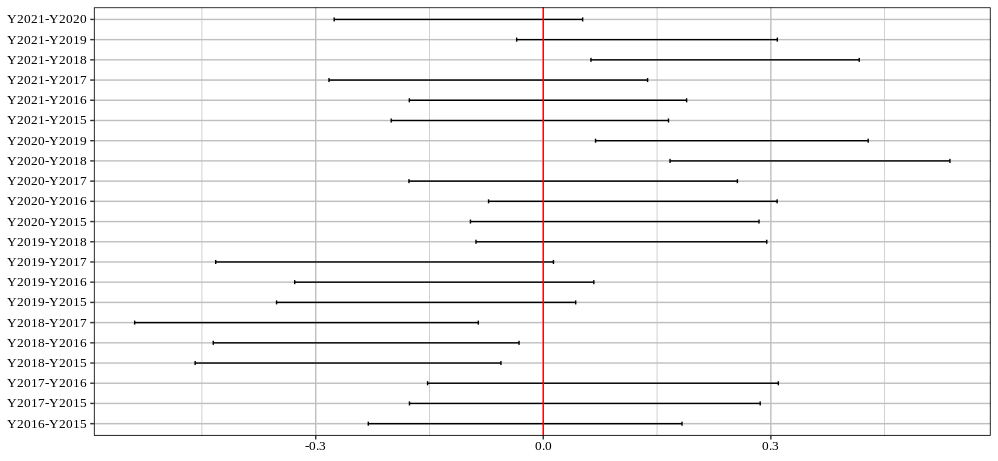
\includegraphics[width=0.80\textwidth]{rendimiento/confidenceot.png}
    \caption{Intervalos de confianza del momento en el que se abre un problema por años.}
    \label{fig:confidencenewcomer}
\end{figure}

\section{Tasa de fallo (fr)}

Podemos ver que la distribución de la tasa de fallo o el número de intentos fallidos para resolver un problema dividido el número de intentos totales de resolución de ese mismo problema se aproxima a una distribución normal, un poco ladeada hacia la derecha a través de su función de densidad (Figura \ref{fig:densityplotfr}) y su gráfico Q-Q (Figura \ref{fig:q-qfr}).

\begin{figure}[H]
    \centering
    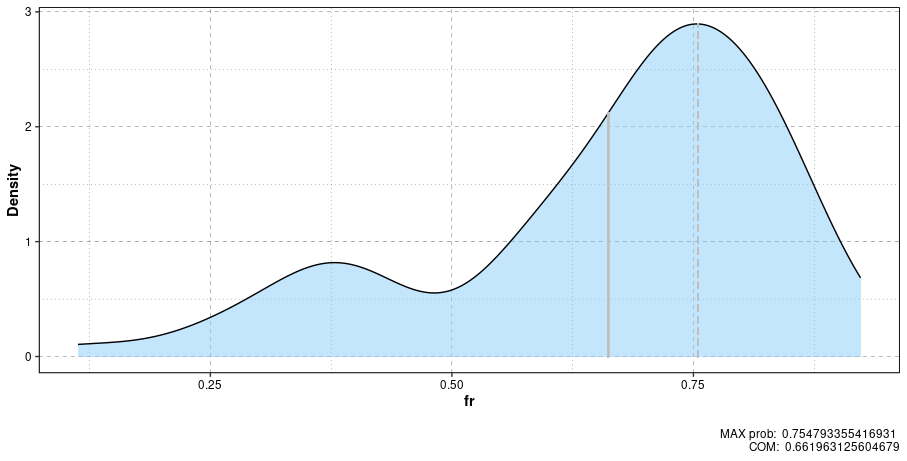
\includegraphics[width=0.70\textwidth]{rendimiento/densityplotfr.png}
    \caption{Función de densidad de probabilidad de la tasa de fallo en la resolución de problemas.}
    \label{fig:densityplotfr}
\end{figure}

\begin{figure}[H]
    \centering
    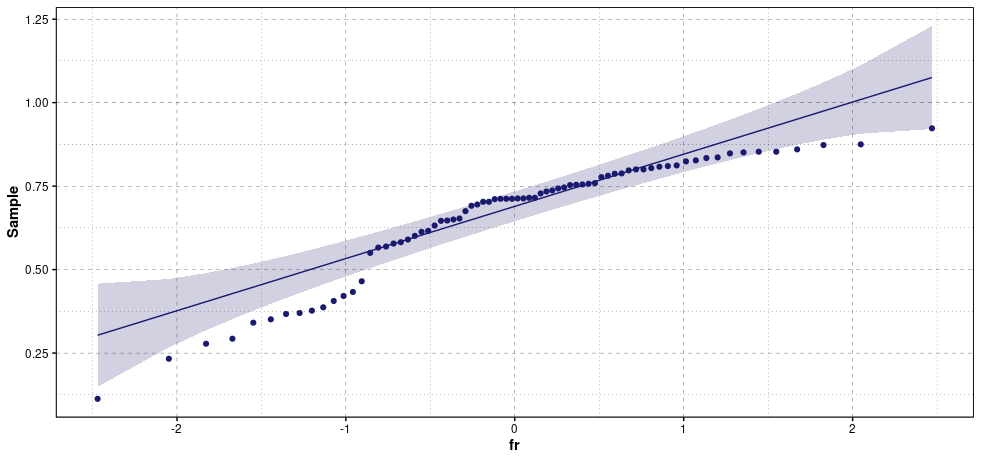
\includegraphics[width=0.75\textwidth]{rendimiento/qqplotfr.png}
    \caption{Gráfico Q-Q de la tasa de fallo en la resolución de problemas.}
    \label{fig:q-qfr}
\end{figure}

En las Figuras \ref{fig:boxplotresidualsfr} y \ref{fig:histogramresidualsfr} podemos ver el boxplot de los residuos de la variable tasa de fallo (\emph{fr}) junto con el histograma de los mismos.

\begin{figure}[H]
\centering
\subfloat[Boxplot de los residuos de la tasa de fallo en la resolución de problemas.]{\label{fig:boxplotresidualsfr}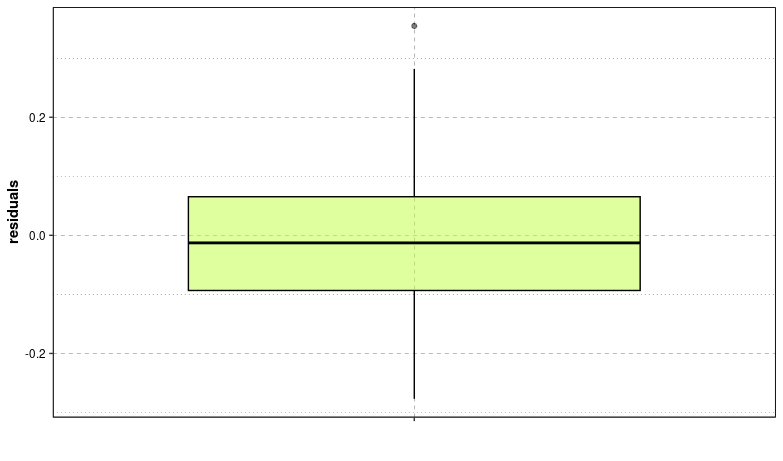
\includegraphics[width=0.47\textwidth]{rendimiento/residualsot.png}}\qquad
\subfloat[Histograma de los residuos de la tasa de fallo en la resolución de problemas.]{\label{fig:histogramresidualsfr}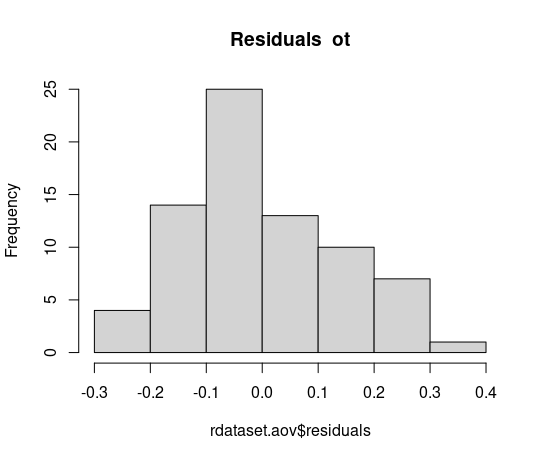
\includegraphics[width=0.47\textwidth]{rendimiento/histogramot.png}}
\caption{Distribución de la tasa de fallo en la resolución de problemas por parte de las diferentes agrupaciones de alumnos.}
\label{fig:fr}
\end{figure}

A continuación, se realizará un estudio por años de la tasa de fallo en la resolución de problemas por parte del alumnado. Como podemos observar en la Figura \ref{fig:boxplotfr}, hay una variación muy perceptible en la tasa de fallo a lo largo de los años. La realización del test ANOVA de un factor, cuyos resultados se muestran en el Cuadro \ref{tab:ANOVAfr}, ratifica que hay diferencias significativas ($p = 6.55e-09 < 0.05$). Igualmente, los resultados del test de Kruskal-Wallis confirman lo anterior ($p-value = 0.0001689 < 0,05$). Posteriormente, se ha realizado el test de Tukey por pares y se ha visto que hay diferencias entre algunos de los cursos académicos considerados (Cuadro \ref{tab:Tukeyfr} y Figura \ref{fig:confidencefr}).

\begin{figure}[H]
    \centering
    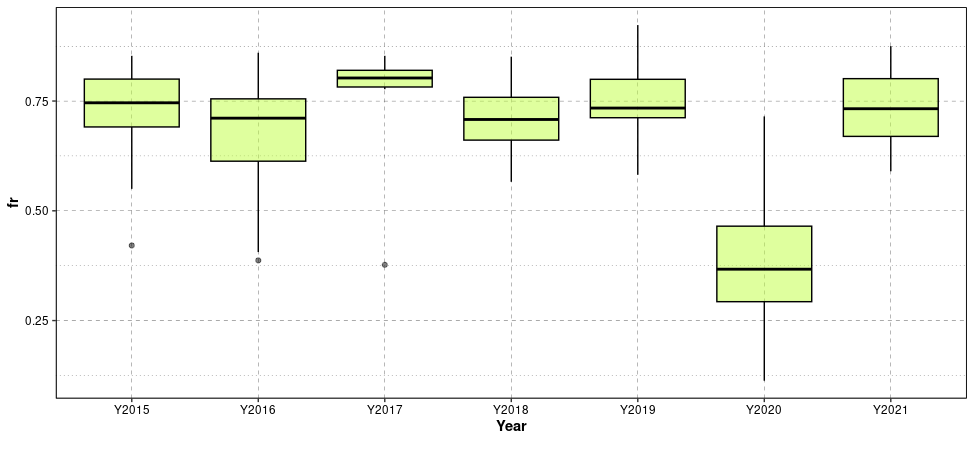
\includegraphics[width=0.8\textwidth]{rendimiento/boxplotfr.png}
    \caption{Boxplot de la tasa de fallo en la resolución de problemas por año.}
    \label{fig:boxplotfr}
\end{figure}

% latex table generated in R 4.3.1 by xtable 1.8-4 package
% Sat Aug  5 18:08:21 2023
\begin{table}[H]
\centering
\caption{Resultados del test ANOVA de un solo factor (tasa de fallo en la resolución de los problemas propuestos).}
\label{tab:ANOVAfr}
\begin{tabular}{lrrrrr}
  \hline
 & Df & Sum Sq & Mean Sq & F value & Pr($>$F) \\ 
  \hline
fr & 6 & 1.19 & 0.20 & 11.68 & 6.55e-09 \\ 
  Residuals        & 67 & 1.14 & 0.02 &  &  \\ 
   \hline
\end{tabular}
\end{table}

% latex table generated in R 4.3.1 by xtable 1.8-4 package
% Sat Aug  5 18:26:09 2023
\begin{table}[H]
\centering
\caption{Test HSD de Tukey (Honestly-significance-difference) de la tasa de fallo en la resolución de los problemas propuestos por año.}
\label{tab:Tukeyfr}
\begin{tabular}{rrrrr}
  \hline
 & diff & lwr & upr & p adj \\ 
  \hline
Y2016-Y2015 & -0.05 & -0.24 & 0.14 & 0.98 \\ 
  Y2017-Y2015 & 0.03 & -0.18 & 0.24 & 1.00 \\ 
  Y2018-Y2015 & 0.00 & -0.18 & 0.19 & 1.00 \\ 
  Y2019-Y2015 & 0.03 & -0.14 & 0.21 & 1.00 \\ 
  Y2020-Y2015 & -0.32 & -0.49 & -0.15 & 0.00 \\ 
  Y2021-Y2015 & 0.03 & -0.14 & 0.19 & 1.00 \\ 
  Y2017-Y2016 & 0.08 & -0.13 & 0.29 & 0.91 \\ 
  Y2018-Y2016 & 0.05 & -0.13 & 0.24 & 0.97 \\ 
  Y2019-Y2016 & 0.08 & -0.09 & 0.26 & 0.78 \\ 
  Y2020-Y2016 & -0.27 & -0.44 & -0.10 & 0.00 \\ 
  Y2021-Y2016 & 0.07 & -0.09 & 0.24 & 0.81 \\ 
  Y2018-Y2017 & -0.03 & -0.23 & 0.18 & 1.00 \\ 
  Y2019-Y2017 & 0.01 & -0.20 & 0.21 & 1.00 \\ 
  Y2020-Y2017 & -0.35 & -0.54 & -0.15 & 0.00 \\ 
  Y2021-Y2017 & -0.00 & -0.19 & 0.19 & 1.00 \\ 
  Y2019-Y2018 & 0.03 & -0.14 & 0.20 & 1.00 \\ 
  Y2020-Y2018 & -0.32 & -0.49 & -0.15 & 0.00 \\ 
  Y2021-Y2018 & 0.02 & -0.14 & 0.18 & 1.00 \\ 
  Y2020-Y2019 & -0.35 & -0.51 & -0.19 & 0.00 \\ 
  Y2021-Y2019 & -0.01 & -0.16 & 0.15 & 1.00 \\ 
  Y2021-Y2020 & 0.34 & 0.19 & 0.49 & 0.00 \\ 
   \hline
\end{tabular}
\end{table}

\begin{figure}[H]
    \centering
    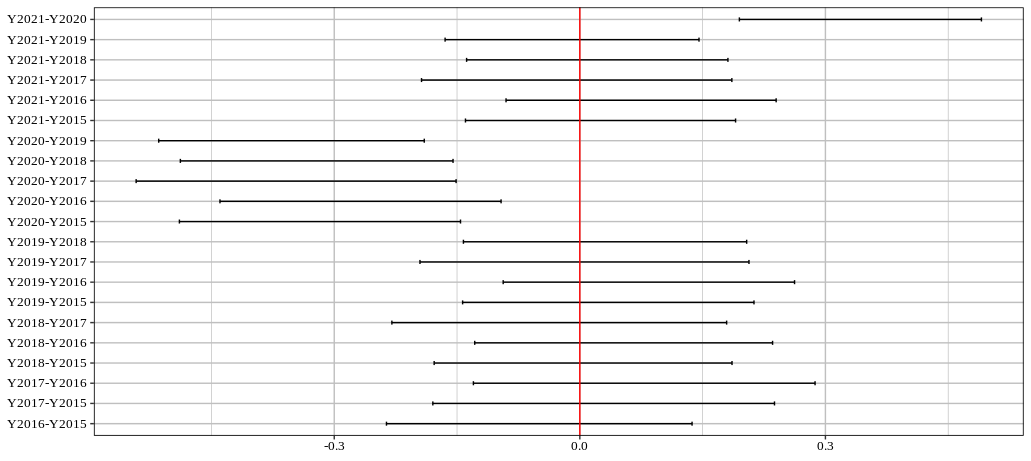
\includegraphics[width=0.80\textwidth]{rendimiento/confidencefr.png}
    \caption{Intervalos de confianza de la tasa de fallo en la resolución de los problemas propuestos por años.}
    \label{fig:confidencefr}
\end{figure}

\section{Tiempo de reacción (\emph{Reaction Time}, rt)}

Tiempo desde que se abre un mismo problema por primera vez hasta que se resuelve normalizado. Este valor está directamente relacionado con la tasa de fallo analizada anteriormente. Podemos ver que esta medida de rendimiento sigue una distribución casi normal, ligeramente inclinada a la izquierda tal y como puede verse en la Figura \ref{fig:densityplotrt}, lo que indica que los grupos suelen emplear poco tiempo en resolver un problema por primera vez.

\begin{figure}[H]
    \centering
    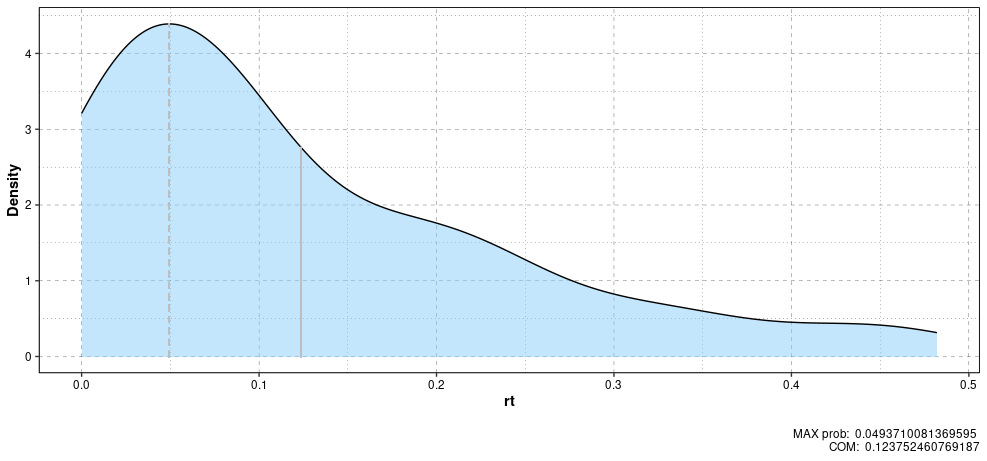
\includegraphics[width=0.70\textwidth]{rendimiento/densityrt.png}
    \caption{Función de densidad de probabilidad del tiempo que los distintos grupos de prácticas dedican a la resolución de problemas desde que se abren por primera vez.}
    \label{fig:densityplotrt}
\end{figure}

Sin embargo, podemos ver que hay algunos grupos que emplean muy pocos intentos para resolver un problema o que, por el contrario, emplean más intentos que la mayoría (Figuras \ref{fig:boxplotresidualssessionsbefore} y \ref{fig:histogramresidualssessionsbefore}).

\begin{figure}[H]
\centering
\subfloat[Boxplot de los residuos del número de intentos necesarios para resolver los problemas por primera vez normalizado.]{\label{fig:boxplotresidualssessionsbefore}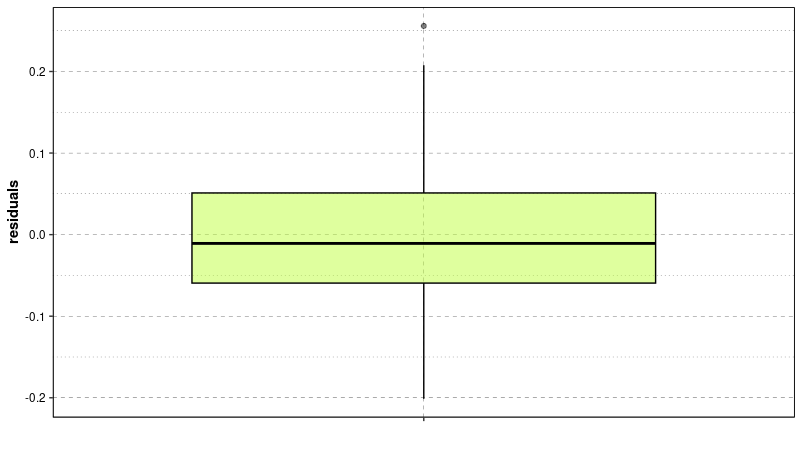
\includegraphics[width=0.47\textwidth]{rendimiento/residualsrt.png}}\qquad
\subfloat[Histograma de los residuos del número de intentos necesarios para resolver los problemas por primera vez normalizado.]{\label{fig:histogramresidualssessionsbefore}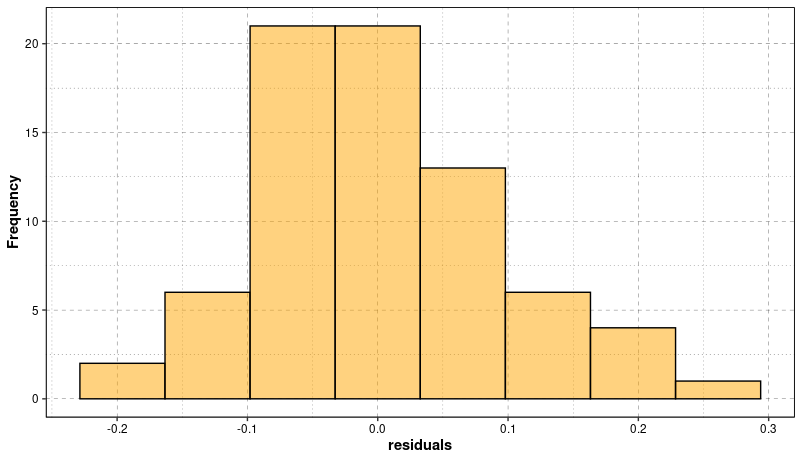
\includegraphics[width=0.47\textwidth]{rendimiento/histogramrt.png}}
\caption{Distribución de los residuos del número de intentos necesarios para resolver los problemas por primera vez normalizado.}
\label{fig:sessionsbefore}
\end{figure}

No obstante, podemos considerar que la regresión es aceptable (Figura \ref{fig:q-qsessionsbefore}).

\begin{figure}[H]
    \centering
    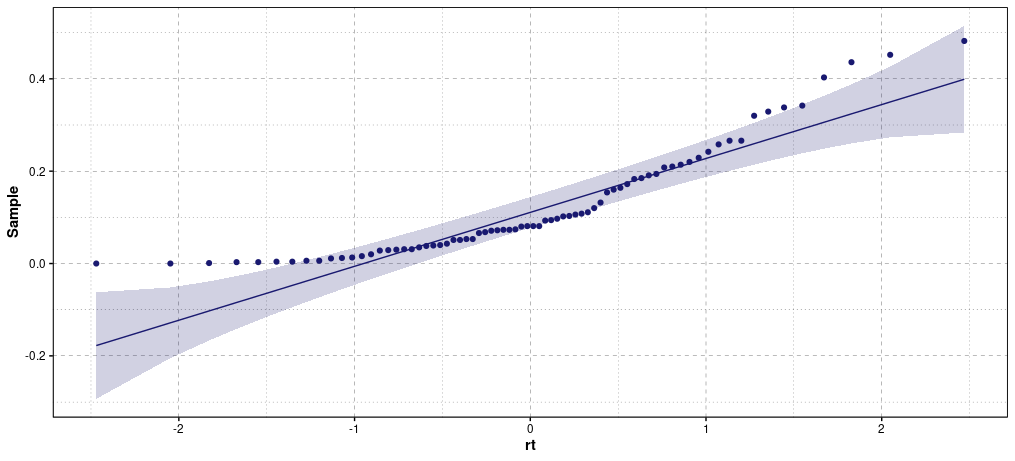
\includegraphics[width=0.75\textwidth]{rendimiento/qqplotrt.png}
    \caption{Gráfico Q-Q del número de intentos necesarios para resolver los problemas por primera vez normalizado.}
    \label{fig:q-qsessionsbefore}
\end{figure}

A continuación, se realizará un estudio por años del número de intentos antes de resolver un problema la primera vez realizados. Como podemos observar en la Figura \ref{fig:boxplotsessionsbefore}, hay una variación muy perceptible en el número de intentos realizados a lo largo de los años. La realización del test ANOVA de un factor (resultados en el Cuadro \ref{tab:ANOVAsessionsbefore}) ratifica que hay diferencias significativas ($p = 8.85e-07 < 0.05$). Igualmente, los resultados del test de Kruskal-Wallis confirman lo anterior ($p-value = 9.767e-07 < 0.05$). Posteriormente, se ha realizado el test de Tukey por pares y se ha visto que hay diferencias entre algunos de los cursos académicos considerados (Cuadro \ref{tab:Tukeysessionsbefore}). Esto mismo puede observarse en la Figura \ref{fig:confidencesessionsbefore}.

\begin{figure}[H]
    \centering
    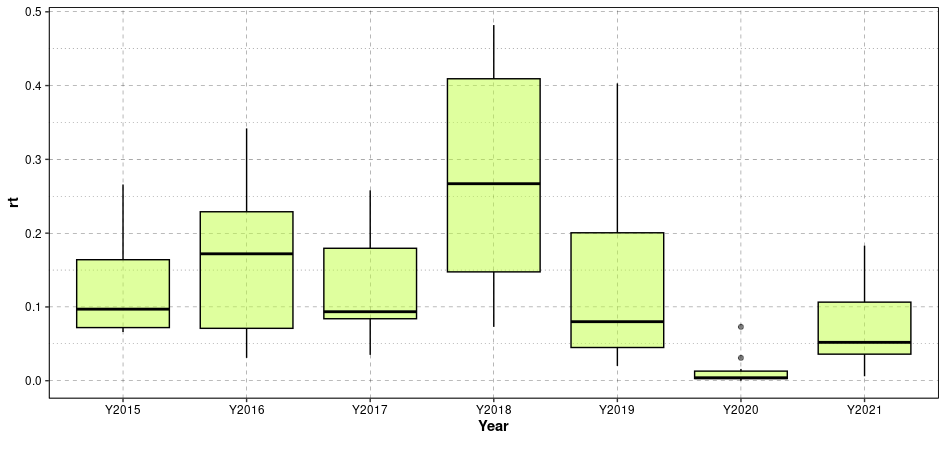
\includegraphics[width=0.8\textwidth]{rendimiento/boxplotrt.png}
    \caption{Boxplot del número de intentos para resolver un problema por año.}
    \label{fig:boxplotsessionsbefore}
\end{figure}

% latex table generated in R 4.3.0 by xtable 1.8-4 package
% Fri Jun  9 10:44:07 2023
\begin{table}[H]
\centering
\caption{Resultados del test ANOVA de un solo factor (número de intentos necesarios para resolver un problema por primera vez normalizado).}
\label{tab:ANOVAsessionsbefore}
\begin{tabular}{lrrrrr}
  \hline
 & Df & Sum Sq & Mean Sq & F value & Pr($>$F) \\ 
  \hline
rt & 6 & 0.45 & 0.07 & 8.37 & 8.85e-07 \\ 
  Residuals        & 67 & 0.60 & 0.01 &  &  \\ 
   \hline
\end{tabular}
\end{table}

% latex table generated in R 4.3.0 by xtable 1.8-4 package
% Fri Jun  9 10:44:35 2023
\begin{table}[H]
\centering
\caption{Test HSD de Tukey (Honestly-significance-difference) del número de intentos realizados para resolver un problema normalizado por año.}
\label{tab:Tukeysessionsbefore}
\begin{tabular}{rrrrr}
  \hline
 & diff & lwr & upr & p adj \\ 
  \hline
Y2016-Y2015 & 0.04 & -0.10 & 0.17 & 0.98 \\ 
  Y2017-Y2015 & -0.00 & -0.15 & 0.15 & 1.00 \\ 
  Y2018-Y2015 & 0.15 & 0.01 & 0.28 & 0.02 \\ 
  Y2019-Y2015 & 0.02 & -0.11 & 0.15 & 1.00 \\ 
  Y2020-Y2015 & -0.12 & -0.24 & 0.01 & 0.08 \\ 
  Y2021-Y2015 & -0.05 & -0.17 & 0.07 & 0.81 \\ 
  Y2017-Y2016 & -0.04 & -0.19 & 0.11 & 0.99 \\ 
  Y2018-Y2016 & 0.11 & -0.02 & 0.24 & 0.19 \\ 
  Y2019-Y2016 & -0.02 & -0.15 & 0.11 & 1.00 \\ 
  Y2020-Y2016 & -0.15 & -0.28 & -0.03 & 0.01 \\ 
  Y2021-Y2016 & -0.09 & -0.21 & 0.03 & 0.24 \\ 
  Y2018-Y2017 & 0.15 & -0.00 & 0.29 & 0.06 \\ 
  Y2019-Y2017 & 0.02 & -0.13 & 0.16 & 1.00 \\ 
  Y2020-Y2017 & -0.12 & -0.26 & 0.03 & 0.19 \\ 
  Y2021-Y2017 & -0.05 & -0.19 & 0.08 & 0.90 \\ 
  Y2019-Y2018 & -0.13 & -0.25 & -0.00 & 0.05 \\ 
  Y2020-Y2018 & -0.26 & -0.38 & -0.14 & 0.00 \\ 
  Y2021-Y2018 & -0.20 & -0.32 & -0.08 & 0.00 \\ 
  Y2020-Y2019 & -0.13 & -0.25 & -0.02 & 0.02 \\ 
  Y2021-Y2019 & -0.07 & -0.19 & 0.04 & 0.45 \\ 
  Y2021-Y2020 & 0.06 & -0.05 & 0.17 & 0.58 \\ 
   \hline
\end{tabular}
\end{table}

\begin{figure}[H]
    \centering
    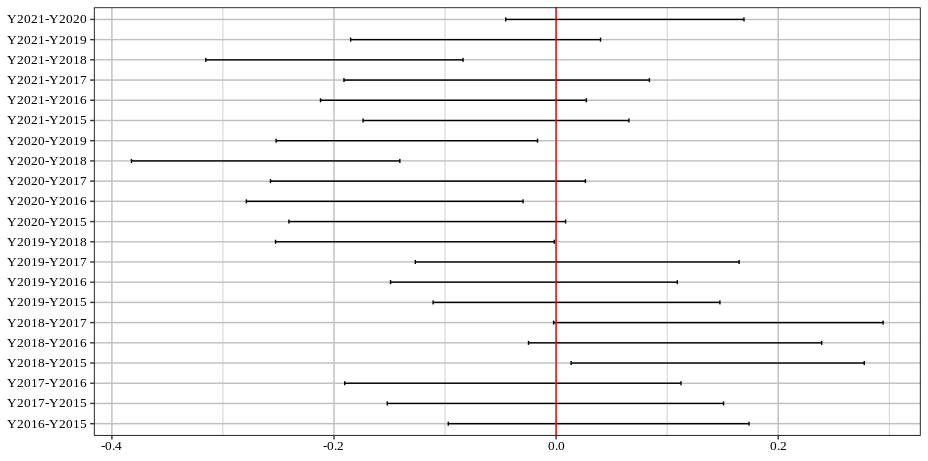
\includegraphics[width=0.80\textwidth]{rendimiento/confidencert.png}
    \caption{Intervalos de confianza del número de intentos antes de resolver un problema normalizado por años.}
    \label{fig:confidencesessionsbefore}
\end{figure}

\section{Perseverancia (ps)}

Curiosamente, algunos grupos siguen trabajando en un problema que ya han resuelto (Figura \ref{fig:densityplotps}).

\begin{figure}[H]
    \centering
    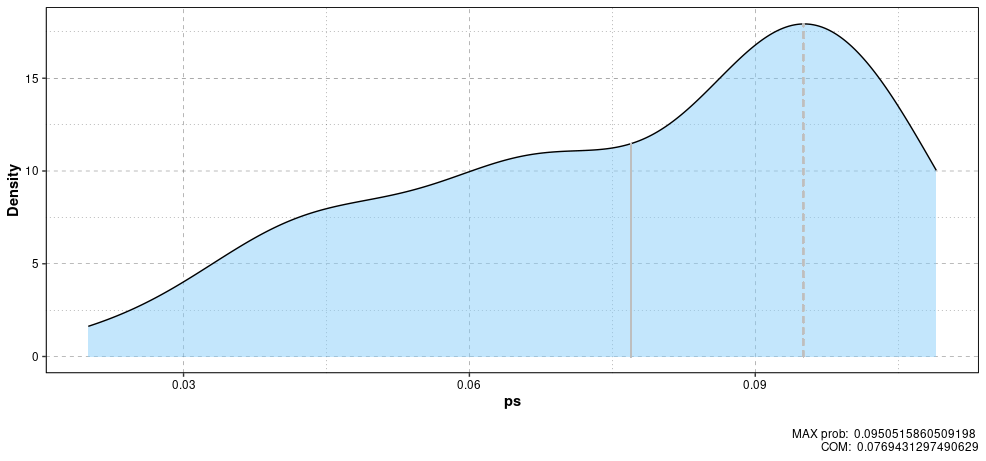
\includegraphics[width=0.70\textwidth]{rendimiento/densityps.png}
    \caption{Función de densidad de probabilidad del tiempo que los distintos grupos de prácticas emplean en un problema tras su resolución.}
    \label{fig:densityplotps}
\end{figure}

\section{Tiempo de comienzo (\emph{Start Time}, st)}

Tiempo transcurrido desde el inicio de las clases hasta que se consigue resolver cada problema por primera vez, normalizado para poder compararlo (ya que la duración de la práctica no es la misma todos los años). Como podemos ver en la Figura \ref{fig:densityplotearlybird}, sigue una distribución casi normal, ladeada hacia la derecha ya que los distintos grupos tienden a resolver los problemas por primera vez al final de la práctica.

\begin{figure}[H]
    \centering
    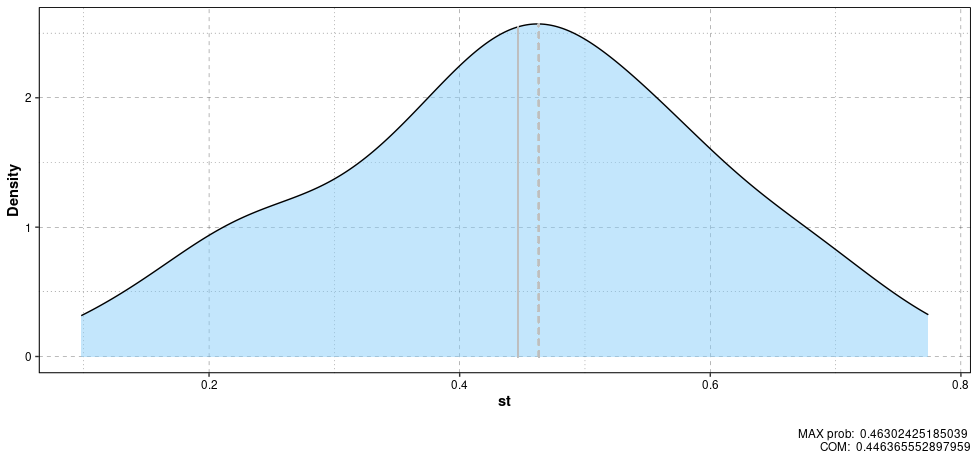
\includegraphics[width=0.70\textwidth]{rendimiento/densityst.png}
    \caption{Función de densidad de probabilidad del momento en el que los distintos grupos de prácticas resuelven por primera vez un problema.}
    \label{fig:densityplotearlybird}
\end{figure}

Podemos observar que no hay presencia de outliers (Figuras \ref{fig:boxplotresidualsearlybird} y \ref{fig:histogramresidualsearlybird}).

\begin{figure}[H]
\centering
\subfloat[Boxplot de los residuos del momento en el que se resuelven los problemas por primera vez normalizado.]{\label{fig:boxplotresidualsearlybird}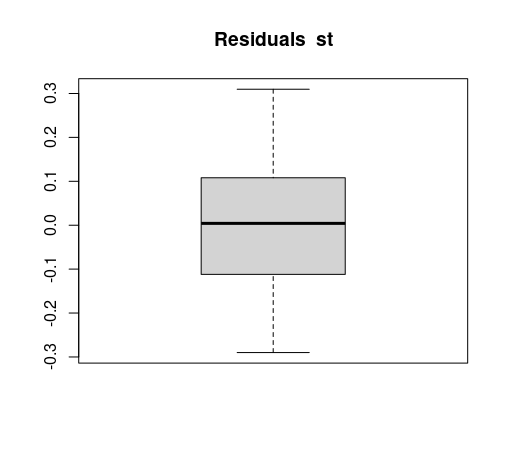
\includegraphics[width=0.47\textwidth]{rendimiento/residualsst.png}}\qquad
\subfloat[Histograma de los residuos del momento en el que se resuelven los problemas por primera vez normalizado.]{\label{fig:histogramresidualsearlybird}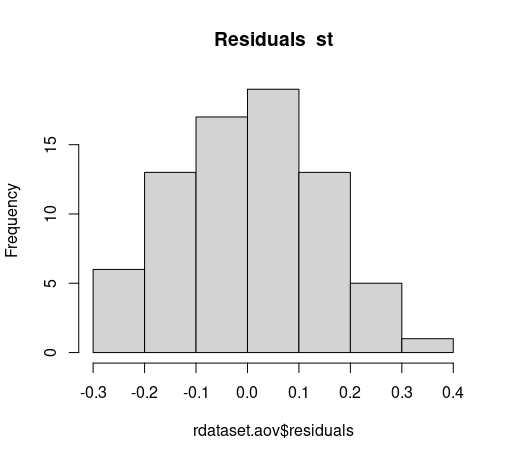
\includegraphics[width=0.47\textwidth]{rendimiento/histogramst.png}}
\caption{Distribución de los residuos del número de intentos desde el comienzo de la práctica hasta la resolución de los problemas por primera vez normalizado.}
\label{fig:earlybird}
\end{figure}

Si se realiza una segmentación por años, intuimos que esta medida de rendimiento sigue la misma distribución de probabilidad todos los cursos académicos estudiados (Figura \ref{fig:boxplotearlybird}). Esto se confirma tras la realización del test ANOVA de un solo factor (Cuadro \ref{tab:ANOVAearlybird}) en el que obtenemos $p = 0.1387 > 0.05$. Realizando el test de Kruskal-Wallis llegamos a la misma conclusión ($p-value = 0.2627$). Además, el test de Tukey muestra que no hay diferencias entre los años considerados (Cuadro \ref{tab:Tukeyearlybird}).

\begin{figure}[H]
    \centering
    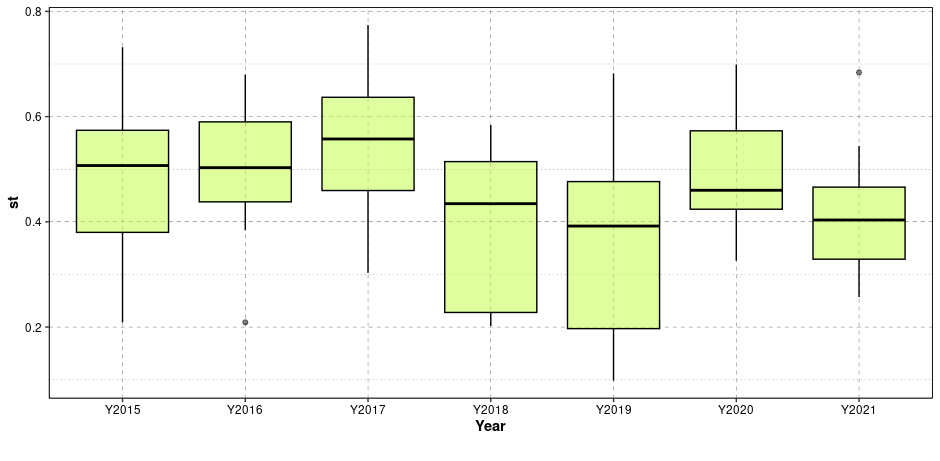
\includegraphics[width=0.8\textwidth]{rendimiento/boxplotst.png}
    \caption{Boxplot del momento en el que se resuelve un problema por primera vez por año.}
    \label{fig:boxplotearlybird}
\end{figure}

% latex table generated in R 4.3.0 by xtable 1.8-4 package
% Sun Jun 11 19:03:22 2023
\begin{table}[H]
\centering
\caption{Resultados del test ANOVA de un solo factor (momento en el que se resuelve un problema por primera vez normalizado).}
\label{tab:ANOVAearlybird}
\begin{tabular}{lrrrrr}
  \hline
 & Df & Sum Sq & Mean Sq & F value & Pr($>$F) \\ 
  \hline
st & 6 & 0.22 & 0.04 & 1.68 & 0.1387 \\ 
  Residuals            & 67 & 1.46 & 0.02 &  &  \\ 
   \hline
\end{tabular}
\end{table}

% latex table generated in R 4.3.0 by xtable 1.8-4 package
% Sun Jun 11 19:03:51 2023
\begin{table}[H]
\centering
\caption{Test HSD de Tukey (Honestly-significance-difference) del momento en el que se resuelve un problema por primera vez normalizado, por año.}
\label{tab:Tukeyearlybird}
\begin{tabular}{rrrrr}
  \hline
 & diff & lwr & upr & p adj \\ 
  \hline
Y2016-Y2015 & 0.02 & -0.19 & 0.23 & 1.00 \\ 
  Y2017-Y2015 & 0.07 & -0.17 & 0.31 & 0.97 \\ 
  Y2018-Y2015 & -0.09 & -0.29 & 0.12 & 0.86 \\ 
  Y2019-Y2015 & -0.11 & -0.31 & 0.10 & 0.69 \\ 
  Y2020-Y2015 & 0.01 & -0.19 & 0.20 & 1.00 \\ 
  Y2021-Y2015 & -0.06 & -0.25 & 0.13 & 0.95 \\ 
  Y2017-Y2016 & 0.05 & -0.19 & 0.28 & 1.00 \\ 
  Y2018-Y2016 & -0.11 & -0.31 & 0.10 & 0.69 \\ 
  Y2019-Y2016 & -0.13 & -0.33 & 0.08 & 0.48 \\ 
  Y2020-Y2016 & -0.01 & -0.21 & 0.18 & 1.00 \\ 
  Y2021-Y2016 & -0.08 & -0.27 & 0.10 & 0.82 \\ 
  Y2018-Y2017 & -0.16 & -0.39 & 0.08 & 0.40 \\ 
  Y2019-Y2017 & -0.17 & -0.40 & 0.05 & 0.25 \\ 
  Y2020-Y2017 & -0.06 & -0.28 & 0.16 & 0.98 \\ 
  Y2021-Y2017 & -0.13 & -0.35 & 0.08 & 0.51 \\ 
  Y2019-Y2018 & -0.02 & -0.21 & 0.18 & 1.00 \\ 
  Y2020-Y2018 & 0.09 & -0.09 & 0.28 & 0.73 \\ 
  Y2021-Y2018 & 0.02 & -0.16 & 0.21 & 1.00 \\ 
  Y2020-Y2019 & 0.11 & -0.07 & 0.30 & 0.51 \\ 
  Y2021-Y2019 & 0.04 & -0.13 & 0.22 & 0.99 \\ 
  Y2021-Y2020 & -0.07 & -0.24 & 0.10 & 0.86 \\ 
   \hline
\end{tabular}
\end{table}

Por último, el análisis de los intervalos de confianza se muestra en la Figura \ref{fig:confidenceearlybird}.

\begin{figure}[H]
    \centering
    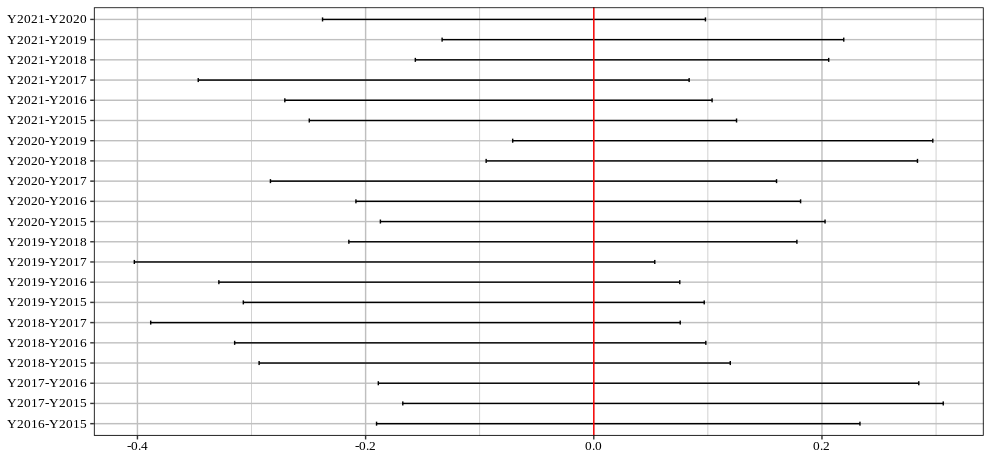
\includegraphics[width=0.80\textwidth]{rendimiento/confidencest.png}
    \caption{Intervalos de confianza del momento en el que se resuelve un problema por primera vez normalizado, por años.}
    \label{fig:confidenceearlybird}
\end{figure}

\section{Siguiendo el plan del profesor (sq)}

Se incorpora una medida de similaridad, en este caso la medida de similaridad del coseno (a la que denotaremos por \emph{sq}), que cuantifica cómo se parece el patrón encontrado con respecto al patrón esperado. En un principio, el profesor espera que los problemas se resuelvan en orden de dificultad creciente (\texttt{P1} \texttt{P2} \texttt{P3} \texttt{P4} \texttt{P5} \texttt{P6} \texttt{P7} \texttt{P8} \texttt{P9}). No obstante, tras el análisis detallado de los registros almacenados, encontramos que muchos grupos optan por resolver los problemas siguiendo un orden diferente al propuesto (por ejemplo, el orden \texttt{P1} \texttt{P3} \texttt{P4} \texttt{P5} \texttt{P7} \texttt{P2} \texttt{P6} \texttt{P8} \texttt{P9}).

La medida de similaridad del coseno se define sobre dos vectores definidos sobre un espacio prehilbertiano\footnote{Espacio vectorial provisto de un producto escalar.}. Así pues, la medida de similaridad del coseno es el coseno del ángulo entre los vectores. Es decir, es el producto escalar de los vectores dividido por el producto de sus longitudes (Ecuación \ref{eq:cosinesimilarity}, donde $A$ y $B$ son dos vectores $n$ dimensionales representando la sucesión de resolución de $n$ problemas de dos grupos de prácticas). De ello se deduce que la semejanza coseno no depende de las magnitudes de los vectores, sino sólo de su ángulo. En la Figura \ref{fig:cosinesimilarity} se representa gráficamente la situación descrita.

\begin{figure}[H]
    \centering
    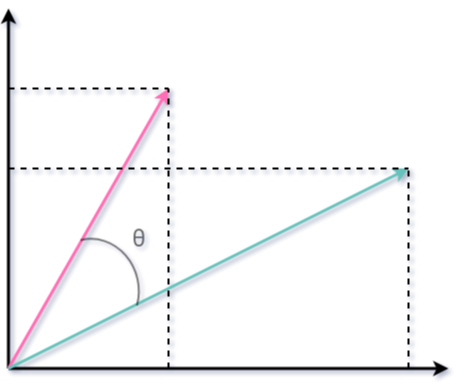
\includegraphics[width=0.35\textwidth]{rendimiento/similaridadcosenoconsombra.png}
    \caption{Representación gráfica del ángulo entre dos vectores con magnitudes positivas en un espacio prehilbertiano de dimensión dos.}
    \label{fig:cosinesimilarity}
\end{figure}

\begin{equation}
\text{cosine similarity }(A,B) = \frac{A\cdot B}{\left\lVert A \right\rVert \cdot \left\lVert B \right\rVert} = \frac{\sum_{i=1}^n {A_i \cdot B_i}}{\sqrt{\sum_{i=1}^n{A_i^2} \cdot \sum_{i=1}^n {B_i^2}}}
\label{eq:cosinesimilarity}
\end{equation}

Trivialmente, la similitud coseno pertenece siempre al intervalo $[-1,1]$. Por ejemplo, dos vectores proporcionales tienen una similitud coseno de $1$, dos vectores ortogonales tienen una similitud de $0$ y dos vectores opuestos tienen una similitud de $-1$. Sin embargo, en nuestro contexto, como los valores componentes de los vectores no pueden ser negativos (serán números naturales entre el uno y el nueve representando a cada uno de los problemas), la semejanza coseno está acotada en el intervalo $[0,1]$.

Nótese que se podría haber definido una medida de similaridad basada en la distancia euclídea. Sin embargo, ésta sólo es de utilidad en espacios de dimensiones pequeñas.

En la Figura \ref{fig:densityplotsq} podemos ver la función de densidad de probabilidad de la medida de rendimiento que estamos considerando.

\begin{figure}[H]
    \centering
    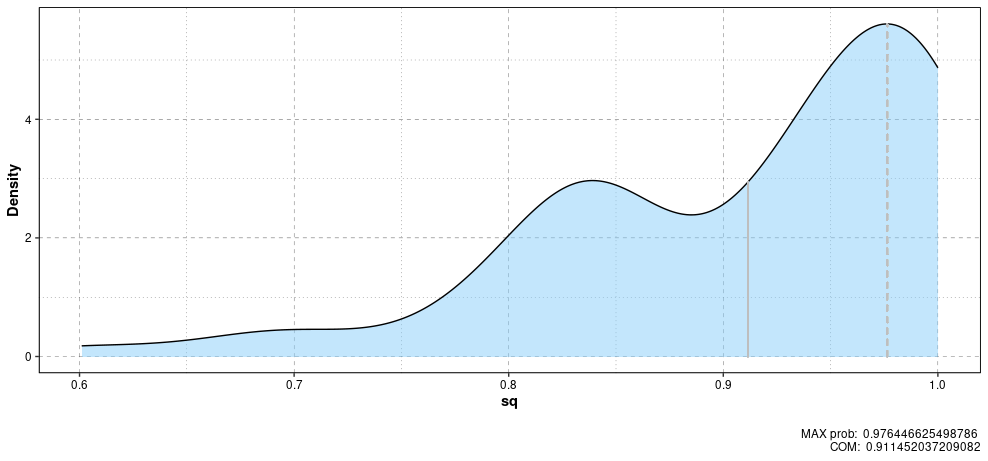
\includegraphics[width=0.70\textwidth]{rendimiento/densitysq.png}
    \caption{Función de densidad de probabilidad del seguimiento del orden de resolución previsto por el profesor que realizan los diferentes grupos de prácticas.}
    \label{fig:densityplotsq}
\end{figure}